\documentclass[12pt,a4paper]{report}
\usepackage[croatian]{babel}
\usepackage[utf8]{inputenc}
\usepackage{amsmath}
\usepackage[margin=3cm]{geometry}
\usepackage{amsfonts}
\usepackage{amssymb}
\usepackage{graphicx}
\usepackage{url}
\usepackage{wrapfig}
\usepackage[table]{xcolor}
\definecolor{lightgray}{gray}{0.9}
\usepackage[hidelinks]{hyperref}
\usepackage{subcaption}
\usepackage{float}
\usepackage{listings}
\usepackage{pgfplots}
\usepackage{cite}
%\renewcommand{\familydefault}{\sfdefault}

\author{Matea Novak \and Filip Novački}
\title{Linearni splajn. Po dijelovima kubična interpolacija}
\begin{document}
	\maketitle
	
	\tableofcontents
	
\chapter{Uvod}
	Ovo je timski projektni zadatak napravljen je u sklopu kolegija Odabrana poglavlja matematike na Fakultetu organizacije i informatike u Varaždinu Sveučilišta u Zagrebu. Cijeli projekt razvijan je na \texttt{git} repozitoriju koji je dostupan na: \url{https://github.com/filipnovacki/linearni-splajn}. 
\chapter{Zadaci}
	\section{Opis glavne ideje po dijelovima polinomne interpolacije}
	Kod raznih mjerenja, istraživanja i sl. se događa da rezultati nekog testiranja budu podaci koji su diskretni, odnosno izmjereni su za neke vrijednosti. Kako bi nam te vrijednosti bile korisne i primjenjive, moramo na neki način odrediti koje su vrijednosti između dviju diskretnih vrijednosti. Tu u priču dolazi interpolacija.
	
	\begin{wrapfigure}{r}{0.55\textwidth}
		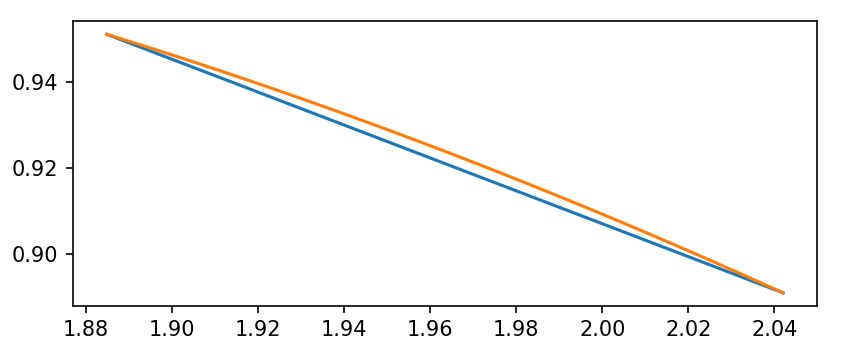
\includegraphics[width=0.55\textwidth]{slike/usporedba.png}
		\caption{Usporedba linearne interpolacije na isječku funkcije $f(x)=\sin x$. Plavom bojom je prikazana interpolacija, a narančastom funkcija. Izvor: autorska izrada}
		\label{usporedba}
	\end{wrapfigure}
	
	Jedna je opcija napraviti interpolaciju linijama prvog reda, dakle, pravcima, odnosno dužinama koje jednostavno povučemo između dviju točaka. Takva aproksimacija je vrlo jednostavna za izračunati, međutim, takvo mjerenje ne daje baš zadovoljavajuće rezultate\cite{ChEn2450}. Drugi je problem što mjesta gdje se ti pravci spajaju su \textit{oštri}, odnosno ne postoji glatki prijelaz.
	
	Kao što vidimo na slici \ref{usporedba}, plava linija dosta je dosta blizu narančastoj, no za razne primjene bi ta greška mogla biti prevelika.
	
	Bolja opcija je povezati točke krivuljama višeg reda. Kako bismo dobili glatki prijelaz, moramo paziti da derivacija u točkama uvijek bude jednaka. Kvadratni polinomi se ne koriste jer se kontrola derivacije može napraviti samo na jednom rubu, što znači da bismo samo s jedne strane mogli imati glatki prijelaz. Parabolička interpolacija nema prave fizikalne podloge i to je dodatni razlog da se ne koristi. Ponekad se koristi u računalnoj grafici.\cite{hari} 
	
	Mogu se koristiti i polinomi još višeg reda, međutim oni se nešto teže računaju te funkcije polinoma višeg reda imaju tendenciju na nekim mjestima jako \textit{divljati}, što ponekad može predstavljati problem\cite{ChEn2450}. 
	
	Najčešći oblik interpolacije je po dijelovima kubična interpolacija te ima važnu fizikalnu podlogu\cite{hari}.
	\subsection{Newtonov oblik}
	Newtonova forma\cite{hari} nam je korisna jer lako dodajemo nove točke interpolacije i na taj način povećavamo stupanj interpolacijskog polinoma. 
	
	Neka je $p_{n-1}$ interpolira neku funkciju $f$ u točkama $x_k, k=0,\ldots,n-1$. Neka polinom $p_n$ interpolira funkciju $f$ u istim točkama i još u točki $x_n$. Tada polinom $p_n$ možemo napisati:
	\begin{equation}
		p_n(x)=p_{n-1}(x)+c(x)
		\label{2.1}
	\end{equation}
	U takvom zapisu, $c(x)$ predstavlja korekciju koja je polinom stupnja $n$. Nadalje, točke $x_k$ moraju biti nultočke polinoma $c$. Stoga vrijedi:
	\begin{equation}
		c(x)=a_n(x-x_0)\ldots(x-x_{n-1})
		\label{2.2}
	\end{equation}
	Iz jednadžbi \ref{2.1} i \ref{2.2} zaključujemo:
	\begin{equation}
		f(x_n)=p_n(x_n)=p_{n-1}(x_n)+a_n(x_n-x_0)\ldots(x_n-x_{n-1})
	\end{equation}
	U ovoj jednadžbi $a_n$ je vodeći koeficijent polinoma $c$. To možemo zapisati još i
	\begin{equation}
		a_n=f[x_0, x_1, \ldots, x_n]
	\end{equation}
	%citirati Pred_0910_4b.pdf
	Na kraju, polinom za stupanj veći od prethodnog možemo definirati kao:
	\begin{equation}
		p_n(x)=p_{n-1}(x_n)+(x-x_0)\ldots(x-x_{n-1})f[x_0, x_1, \ldots, x_n]
		\label{2.5}
	\end{equation}
	Rekurzivo, iz izraza \ref{2.5} dobivamo napokon Newtonov oblik interpolacijskog polinoma koji glasi:
	\begin{align*}
	P_i(x)=&f[x_0]\\
	+&f[x_0,x_1](x-x_0)\\
	+&f[x_0,x_1,x_2](x-x_0)(x-x_1)\\
	+&f[x_0,x_1,x_2,x_3](x-x_0)(x-x_1)(x-x_2)\\
	+&\ldots+f[x_0,x_1,\ldots,x_n](x-x_0)\ldots(x-x_{n-1})
	\end{align*}
	Interpolacijski polinom stupnja 0 je zapravo točka koja interpolira funkciju $f$ u točki $x_0$.
	\begin{equation*}
		P_0(x)=f_0
	\end{equation*}
	Nadalje, interpolacijski polinom stupnja 1 nastaje tako da prethodnom polinomu stupnja 0 dodamo korekciju $c_1$.
	\begin{equation*}
		p_1(x)=p_0(x)+c_1(x)
	\end{equation*}
	Za $f_0$ korekcija $c_1$ mora biti $c_1(x_0)=0$. 
	
	Interpolacijski polinom stupnja 2 nastaje tako da dodamo još jedan čvor interpolacije $x_2$. Sada polinom $p_2$ dobijemo tako da polinomu $p_1$ dodamo korekciju $c_2$\cite{NumMatPrez}.
	\begin{equation*}
		p2(x)=p_1(x)+c_2(x)
	\end{equation*}
	
	\section{Opis linearnog splajna}
	
	Kao što smo već objasnili spajn ranije, on nam služi za dobivanje vrijednosti koji su između dviju izmjerenih vrijednosti.
	
	\begin{minipage}{0.4\textwidth}
	\begin{table}[H]
		\begin{tabular}{c c}
			Godina&Broj stanovnika\\\hline
			2001	&	48068	\\
%			2002	&	47723	\\
%			2003	&	47460	\\
			2004	&	47185	\\
%			2005	&	47050	\\
%			2006	&	46972	\\
			2007	&	46968	\\
%			2008	&	46912	\\
%			2009	&	46902	\\
			2010	&	46957	\\
%			2011	&	46938	\\
%			2012	&	46781	\\
			2013	&	46574	\\
%			2014	&	46476	\\
%			2015	&	46319	\\
			2016	&	46294	\\
			
		\end{tabular}
	\caption{Izvor: \url{www.dzs.hr}}
	\label{dzsStan}
	\end{table}
	\end{minipage}
	\begin{minipage}{0.6\textwidth}
		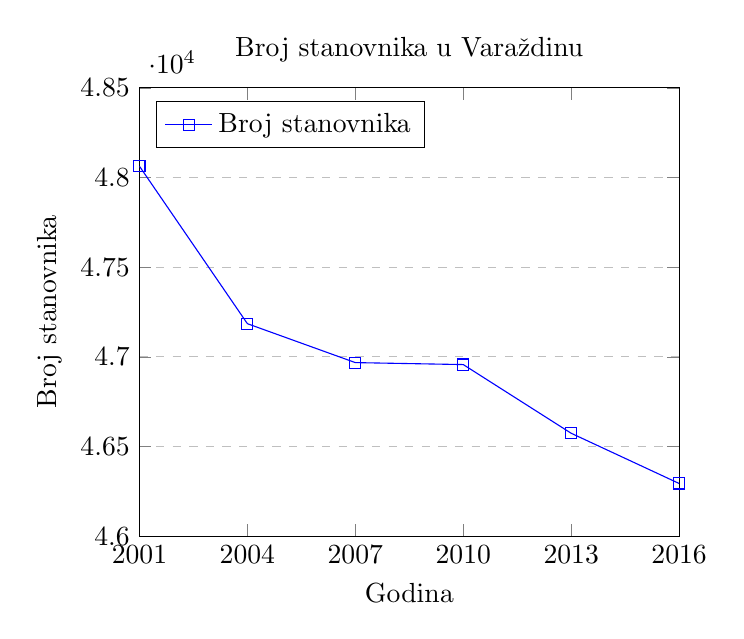
\begin{tikzpicture}
		\begin{axis}[
		title={Broj stanovnika u Varaždinu},
		x tick label style={
			/pgf/number format/1000 sep=},
		xlabel={Godina},
		ylabel={Broj stanovnika},
		xmin=2001, xmax=2016,
		ymin=46000, ymax=48500,
		xtick={2001, 2004, 2007, 2010, 2013, 2016},
		ytick={46000, 46500, 47000, 47500, 48000, 48500},
		legend pos=north west,
		ymajorgrids=true,
		grid style=dashed,
		]
		
		\addplot[
		color=blue,
		mark=square,
		]
		coordinates {
			(2001,48063)
%			(2002,47723)
%			(2003,47460)
			(2004,47185)
%			(2005,47050)
%			(2006,46972)
			(2007,46968)
%			(2008,46912)
%			(2009,46902)
			(2010,46957)
%			(2011,46938)
%			(2012,46781)
			(2013,46574)
%			(2014,46476)
%			(2015,46319)
			(2016,46294)
		};
		\legend{Broj stanovnika}
		
		\end{axis}
		%
		\end{tikzpicture}

	
	\end{minipage}
	Pogledajmo tablicu \ref{dzsStan} i pripadni graf. U ovim podacima vidimo popise stanovništa za svaku treću godinu. Linearni splajn bi nam ovdje pomogao da prepostavimo koliko je moglo biti stanovnika između dvaju izmjerenih razdoblja.
	
	Prednosti linearnog splajna su što vrlo jednostavne za izračunati za bilo koju točku, kao što ćemo vidjeti u primjerima. Glavni nedostatak linearne interpolacije je to što može doći do značajnih odstupanja kod nelinearnih funkcija koji su česti u fizici, kemiji i sl.
	\section{Primjeri}
		\subsection{Algoritam za traženje linearnog splajna}
		Neka je zadana neprekidna funkcija $f:[a,b]\rightarrow \mathbb{R} $ i neka je segment $[a,b]$ podijeljen na $n$ jednakih dijelova, tj. neka su
		\begin{equation*}
			x_i=a+ih,\quad i=0,1,\ldots,n,\quad h=\frac{b-a}{n}
		\end{equation*}
		
		Algoritam koji računa linearni splajn izmađu dvaju ekvidistantnih čvorova $x_i$ započinje pronalaženjem točaka.
		
		\begin{align*}
			y_i&=f(x_i)\\
			y_{i+1}&=f(x_{i+1})\\
			&\downarrow\\
			T_i&(x_i, y_i)\\
			T_{i+1}&(x_{i+1}, y_{i+1})
		\end{align*}
		
		Zatim moramo pronaći pravac koji je razapet između tih dviju točaka. To možemo napraviti po formuli koja je opće poznata\cite{pmfPrezp5}:
		\begin{equation}
		y=\biggr{(}\frac{y_{i+1}-y_i}{x_{i+1}-x_i}\biggr{)}(x-x_i)+y_i
		\label{pravac}
		\end{equation}
		
		
		\subsection{$f(x)=\sin x$}
			Ovaj ćemo zadatak riješiti za $i=1, 2,\ldots, 40$. S obzirom da nema nekog smisla pisati za svaki interval pojedinačno, ovaj ćemo zadatak riješiti programskim putem, a ručno ćemo pokazati samo na jednom primjeru. Tablicu s rješenjima možemo vidjeti u tablici \ref{linInterpolTablica}.
			\begin{align*}
				f(x)=\sin (x),& \quad x\in [0, 2\pi]\\
				n&=40\\
				a&=0\\
				b&=2\pi\\
			\end{align*}
			Pronađimo prva dva čvora. %Pri računanju koristimo \texttt{Python}:
%	
%			\begin{lstlisting}
%Python 3.6.3 (default, Oct  3 2017, 21:45:48) 
%[GCC 7.2.0] on linux
%Type "help", "copyright", "credits" or "license" for more information.
%>>> import numpy as np
%>>> b = 2 * np.pi
%>>> a = 0
%>>> n = 40
%>>> h = (b - a) / n
%>>> 
%>>> x0 = a + 0 * h
%>>> y0 = np.sin(x0)
%>>> x1 = a + 1 * h
%>>> y1 = np.sin(x1)
%>>> x0
%0.0
%>>> y0
%0.0
%>>> x1
%0.15707963267948966
%>>> y1
%0.15643446504023087
%			\end{lstlisting}
%	
%			K\^{o}d u prijevodu na matematički jezik glasi ovako:
			\begin{align*}
				x_0=&0\quad\rightarrow \quad y_0=f(0)=0\\
				x_1=&a+ih\\=&0+1\frac{2\pi-0}{40}\\
					=&0.15707963267948966\\
				y_1=&f\biggr{(}\frac{2\pi}{40}\biggr{)}\\=&0.15643446504023087
			\end{align*}
			Uvrštavanjem ovih podataka u jednadžbu \ref{pravac} dobivamo:
			\begin{equation}
				y=1.0041242039539873x
				\label{linInt1}
			\end{equation}
			Kad razmislimo o rješenju, vidimo da ono ima smisla jer prolazi kroz ishodište, a nagib je skoro jednak 1, što također ima smisla jer koordinate točke skoro jednake. Osim toga, i grafički rješenje ima smisla, što možemo vidjeti na slici \ref{linInterSlika1}.
			\begin{figure}[H]
				\centering
				\begin{minipage}{.5\textwidth}
					\centering
					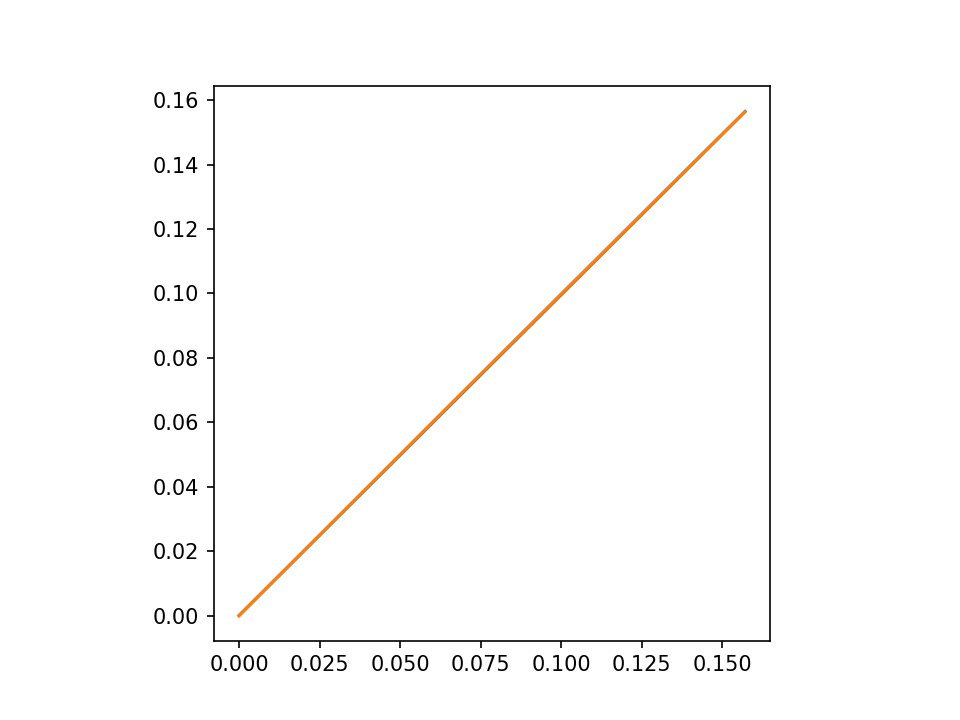
\includegraphics[width=\textwidth]{slike/usporedba40.png}
				\end{minipage}%
				\begin{minipage}{.5\textwidth}
					\centering
					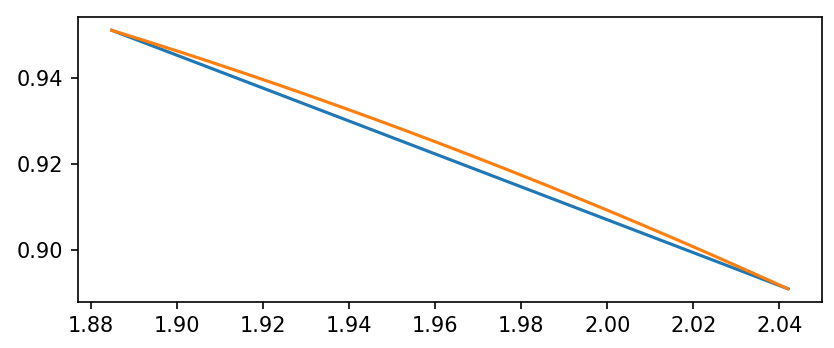
\includegraphics[width=\textwidth]{slike/usporedba412.png}
				\end{minipage}
				\caption{Usporedba funkcije $f(x)=\sin (x)$ i linearne interpolacije po jednadžbi pravca iz jednadžbe \ref{linInt1} te na isječku za $i=13$. Plavom bojom je prikazana interpolacija, a narančastom funkcija. Izvor: autorska izrada}
				\label{linInterSlika1}
			\end{figure}
			Cijela funkcija s pripadnim linearnim interpolacijama izgleda ovako:
			\begin{figure}[H]
				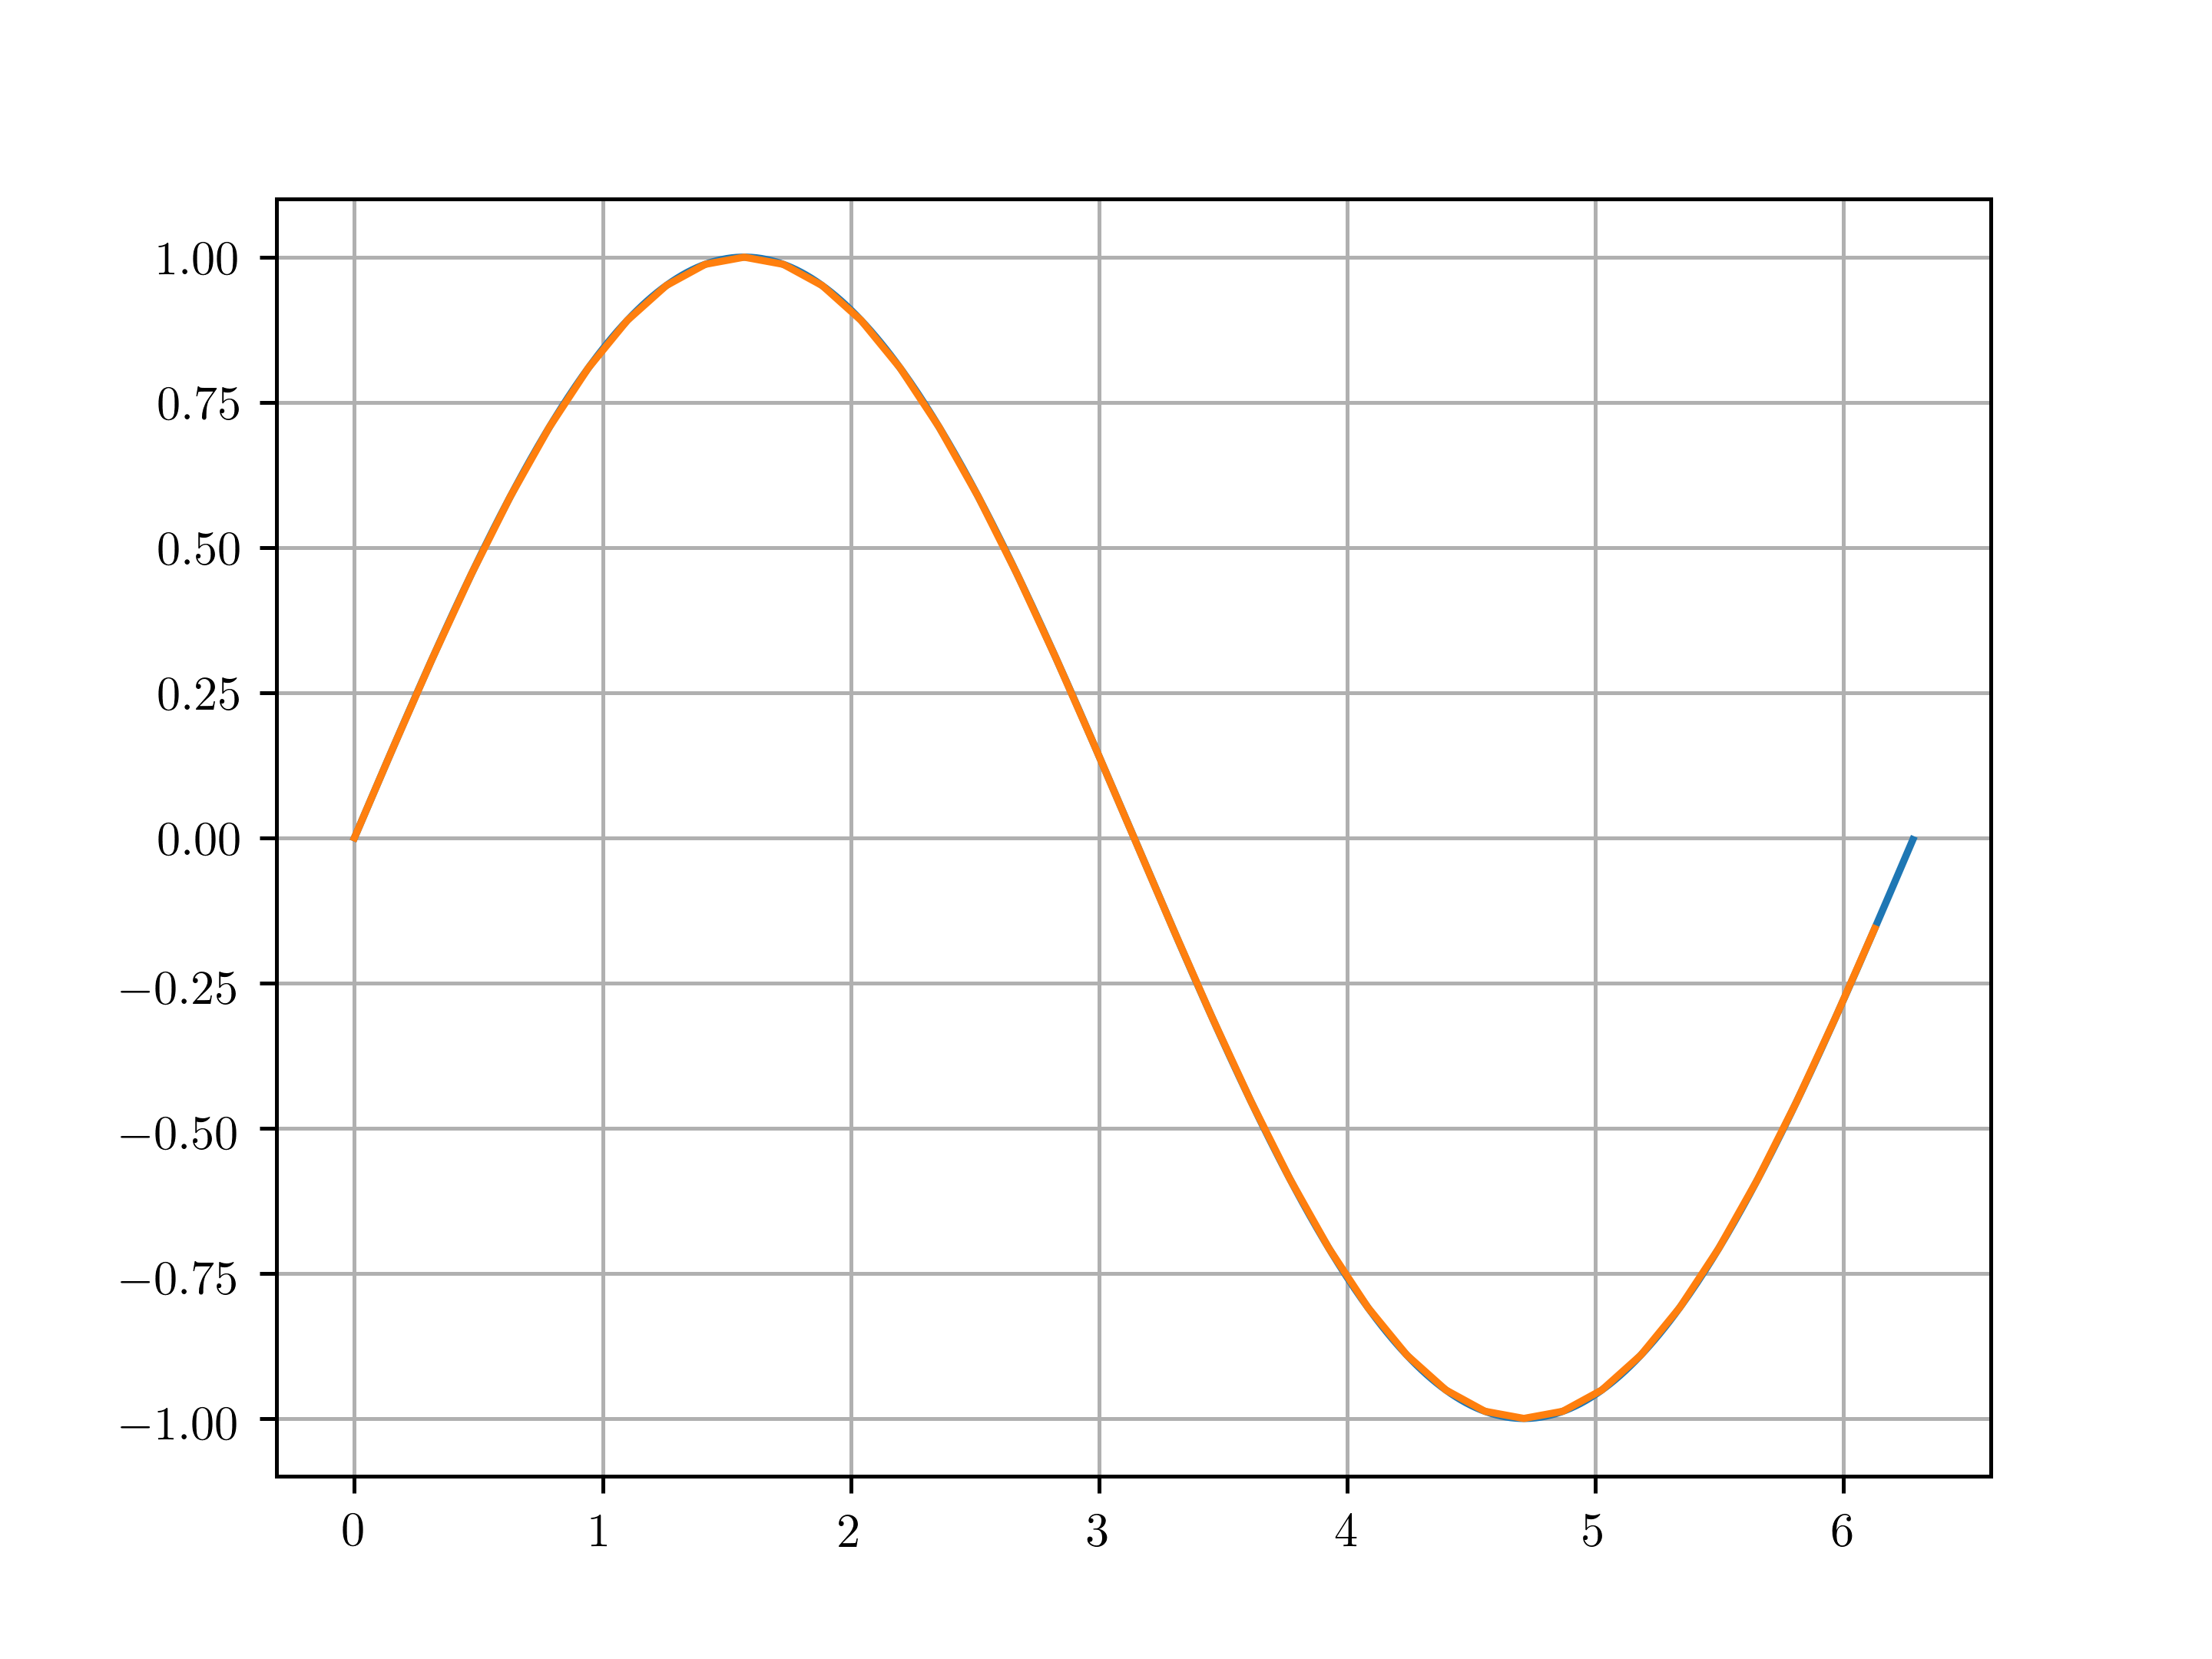
\includegraphics[width=\textwidth]{slike/usporedbaLinearneInterpolacijeSin.png}
				\caption{Prikaz funkcije $f(x)=\sin (x)$ i linearnih interpolacija. Izvor: autorska izrada}
			\end{figure}
		\subsection{$g(x)=\frac{1}{x^2 +1}$}
			Ovaj ćemo zadatak riješiti koristeći isti algoritam kao u prethodnom zadatku. Za početak bismo trebali provjeriti domenu funkcije s obzirom da varijabla $x$ u nazivniku uvijek malo miriše na nevolje i dijeljenje s nulom. Stoga zaključujemo da imamo uvjet $x^2+1\neq0$, zaključujemo da $x^2\neq-1$ te smo sretni jer nam je domena $\mathbb{R}$.
			
			Sad nećemo pokazivati ručne korake, nego ćemo jednostavno programskim putem izračunati ono što nas zanima za navedenu funkciju. Početne postavke su pokazane u nastavku, a rezultati su pokazani u tablici \ref{linInterpolTablicaDva}. Grafički prikaz možemo vidjeti na slici \ref{linInterSlika2}.
			
			\begin{align*}
			g(x)=\frac{1}{x^2 +1},& \quad x\in [-5,5]\\
			n&=40\\
			a&=-5\\
			b&=5\\
			\end{align*}
			
			\begin{figure}[H]
				\centering
				
					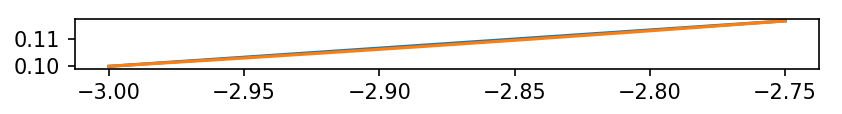
\includegraphics[width=\textwidth]{slike/usporedba58.png}
				
					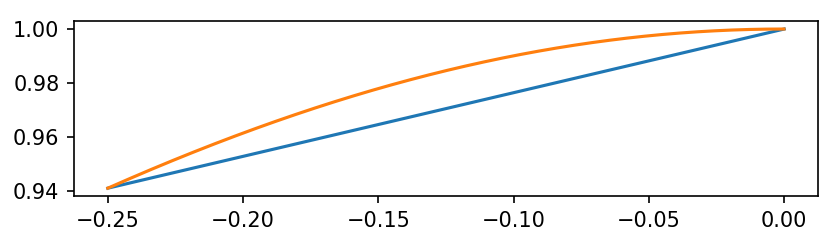
\includegraphics[width=\textwidth]{slike/usporedba519.png}
				
				\caption{Usporedba funkcije $g(x)=\frac{1}{x^2 +1}$ i linearne interpolacije po jednadžbi pravca iz tablice \ref{linInterpolTablicaDva} za $i=9$ te $i=20$. Plavom bojom je prikazana interpolacija, a narančastom funkcija. Izvor: autorska izrada}
				\label{linInterSlika2}
			\end{figure}
			
			
			
	\section{Opis nedostataka linearnih splajnova}
	\section{Opis po dijelovima kubične interpolacije}
	Ideja kubične interpolacije je prikaz neke funkcije pomoću više polinoma trećeg stupnja, svakog na nekom intervalu između dvije krajnje točke.
	
	Kod po dijelovima kubične interpolacije restrikcija aproksimacijske funkcije $f$ na svaki interval $[x_{k-1},x_k]$ je kubični polinom kojeg zapisujemo relativno s obzirom na početnu točku intervala u obliku:
	\begin{align*}
		P_k(x)=C_{0,k}+C_{1,k}(x-x_{k-1})+C_{2,k}(x-x_{k-1})^2+C_{3,k}
		(x-x_{k-1})^3\\
		P_k\in \mathcal{P}_3, x\in [x_{k-1}, x_k], k=1,\ldots,n
	\end{align*}
	
	Kubična se interpolacija koristi zato što je niskog stupnja te je stoga jednostavna za izračun. Unatoč tome, rezultat koji se dobije tim postupkom je zadovoljavajuće točnosti, gladak je i neprekidan u čvorovima.
	
	\section{Primjeri}
		\subsection{Algoritam za traženje po dijelovima kubične interpolacije}
		Postoje dva načina na koje možemo izračunati kubičnu interpolaciju. Prvi je pomoću standardnog oblika (Newtonovog oblika), a drugi pomoću Hermiteove polinomne interpolacije.
		
		Hermiteova polinomna interpolacija izgleda ovako:
		\begin{align*}
		P_i(x)=C_{0,i}+C_{1,i}(x-x_{i-1})+C_{2,i}(x-x_{i-1})^2+C_{3,i}(x-x_{i-1})^3 \\
		x\in[x_{i-1}, x_i], i=1,...,n
		\end{align*}
		Neprekidnost funkcije se osiguravaju na način da interpolacija mora davati iste vrijednosti kao i funkcija u rubovima svog podintervala, odnosno:
		\begin{align*}
			&P_i(x_i)=f_i\\
			&P_i(x_{i-1})=f_{i-1}\\
			%&h_i=x_i-x_{i-1} &f[x_i, x_i]=f'(x_i)=s_i
		\end{align*}
		Kako bi funkcija bila što glađa, potrebno je učiniti derivacije interpolacija jednakim u čvorovima, odnosno:
		\begin{align*}
		P_i'(x_i)=S_i\\
		P_i'(x_{i-1})=S_{i-1}\\
		\end{align*}
		
		
		Za računanje kubične interpolacije možemo koristiti i Newtonov oblik interpolacijskog polinoma. Taj smo oblik već opisali, stoga nećemo diskutirati detalje, nego ćemo opisati kako se može elegantno doći do rješenja. Jednostavnim algoritmom možemo opisati računanje podijeljenih razlika:
		\begin{lstlisting}
for i:=1 to n do
  for j := n to i do
    f[j] := (f[j]-f[j-1])/(x[j]-x[j-1])
		\end{lstlisting}


		\subsection{$f(x)=\sin x$}
		Sad ćemo na primjeru pokazati kako izračunati kubičnu interpolaciju. Primjer je zadan ovako:
		\begin{align*}
			f(x)=\sin x, \quad x\in [0, 2\pi], \quad n=1,...,40.
		\end{align*}
		Za početak, tražimo rješenje za $n=1$. Tada nam je $h=2\pi$. Očekivano, $x_0 = 0$, a $x_1 = 2\pi$.  
		
		Nadalje,
		\begin{align*}
			C_{0,1}&=\frac{P_1(x_0)}{0!}=f(x_0)=\sin (x_0)=\sin (0) = 0\\
			C_{1,1}&=\frac{P'_k(x_0)}{1!}=f'(x_0)=\sin(x_0)'=\cos(0) =1\\
			C_{2, 1}&=\frac{P''_k(x_0)}{2!}=\frac{(\sin (x_0))''}{2}=\frac{-\sin(0)}{2}=0\\
			C_{3, 1}&=\frac{P'''_k(x_0)}{3!}=\frac{(\sin (x_0))'''}{6}=\frac{-\cos(0)}{6}=-\frac{1}{6}\\
		\end{align*}
		Izračunate vrijednosti uvrštavamo u gornju jednadžbu te dobivamo polinom:
		\begin{align*}
			P_i=0+1(x-0)+0(x-0)^2-\frac{1}{6}(x-0)^3 = 1x-\frac{1}{6}x^3
		\end{align*}
		Uvjerimo se u točnost rezultata slikom:
		\begin{figure}[H]
			\centering
			\begin{tikzpicture}% function
			\begin{axis}[axis x line=center, axis y line=center, ymin=-1]
			\addplot[domain=0:2*pi,smooth, color=red] (\x,{sin(\x r)});
			\addplot[domain=0:2*pi,smooth, color=blue]
			(\x,{1*\x-(x^3/6)});
			\end{axis}
			\end{tikzpicture}
			\caption{Prikaz funkcije $f(x)=\sin x$ (crveno) i interpolacije te funkcije polinomom trećeg stupnja $P(x)=1x-\frac{1}{6}x^3$ (plavo)}
		\end{figure}
		\subsection{$g(x)=\frac{1}{x^2 +1}$}
\chapter{Zaključak}
\chapter{Dodatak}
	U ovom poglavlju se nalaze tablice koje bi svojom veličinom kvarile ugodnost čitanja te su stavljene na kraj. Na mjestima gdje su pozvane su napravljene poveznice do njih tako da su jednostavno pristupačne klikom na njih.
		\begin{table}
	\rowcolors{1}{}{lightgray}
	\begin{center}		
		\begin{tabular}{c | c c | c c | c | c}
			$i$&$x_1$&$y_1$&$x_2$&$y_2$&Interpolacija&$\text{Razlika}$\\\hline
			1 &$0.0000$&$0.0000$&$0.1571$&$0.1564$&$y =  0.9959x+0.0000$&$-0.84$\\
			2 &$0.1571$&$0.1564$&$0.3142$&$0.3090$&$y =  0.9714x+0.0039$&$-0.69$\\
			3 &$0.3142$&$0.3090$&$0.4712$&$0.4540$&$y =  0.9229x+0.0191$&$-0.53$\\
			4 &$0.4712$&$0.4540$&$0.6283$&$0.5878$&$y =  0.8518x+0.0526$&$-0.39$\\
			5 &$0.6283$&$0.5878$&$0.7854$&$0.7071$&$y =  0.7596x+0.1105$&$-0.25$\\
			6 &$0.7854$&$0.7071$&$0.9425$&$0.8090$&$y =  0.6488x+0.1976$&$-0.13$\\
			7 &$0.9425$&$0.8090$&$1.0996$&$0.8910$&$y =  0.5220x+0.3171$&$-0.03$\\
			8 &$1.0996$&$0.8910$&$1.2566$&$0.9511$&$y =  0.3823x+0.4707$&$0.05$\\
			9 &$1.2566$&$0.9511$&$1.4137$&$0.9877$&$y =  0.2332x+0.6580$&$0.11$\\
			10 &$1.4137$&$0.9877$&$1.5708$&$1.0000$&$y =  0.0784x+0.8769$&$0.15$\\
			11 &$1.5708$&$1.0000$&$1.7279$&$0.9877$&$y = -0.0784x+1.1231$&$0.16$\\
			12 &$1.7279$&$0.9877$&$1.8850$&$0.9511$&$y = -0.2332x+1.3906$&$0.15$\\
			13 &$1.8850$&$0.9511$&$2.0420$&$0.8910$&$y = -0.3823x+1.6717$&$0.11$\\
			14 &$2.0420$&$0.8910$&$2.1991$&$0.8090$&$y = -0.5220x+1.9569$&$0.05$\\
			15 &$2.1991$&$0.8090$&$2.3562$&$0.7071$&$y = -0.6488x+2.2358$&$-0.03$\\
			16 &$2.3562$&$0.7071$&$2.5133$&$0.5878$&$y = -0.7596x+2.4969$&$-0.13$\\
			17 &$2.5133$&$0.5878$&$2.6704$&$0.4540$&$y = -0.8518x+2.7285$&$-0.25$\\
			18 &$2.6704$&$0.4540$&$2.8274$&$0.3090$&$y = -0.9229x+2.9185$&$-0.39$\\
			19 &$2.8274$&$0.3090$&$2.9845$&$0.1564$&$y = -0.9714x+3.0555$&$-0.53$\\
			20 &$2.9845$&$0.1564$&$3.1416$&$0.0000$&$y = -0.9959x+3.1287$&$-0.69$\\
			21 &$3.1416$&$0.0000$&$3.2987$&$-0.1564$&$y = -0.9959x+3.1287$&$-0.84$\\
			22 &$3.2987$&$-0.1564$&$3.4558$&$-0.3090$&$y = -0.9714x+3.0478$&$-1.00$\\
			23 &$3.4558$&$-0.3090$&$3.6128$&$-0.4540$&$y = -0.9229x+2.8804$&$-1.15$\\
			24 &$3.6128$&$-0.4540$&$3.7699$&$-0.5878$&$y = -0.8518x+2.6233$&$-1.30$\\
			25 &$3.7699$&$-0.5878$&$3.9270$&$-0.7071$&$y = -0.7596x+2.2759$&$-1.43$\\
			26 &$3.9270$&$-0.7071$&$4.0841$&$-0.8090$&$y = -0.6488x+1.8406$&$-1.55$\\
			27 &$4.0841$&$-0.8090$&$4.2412$&$-0.8910$&$y = -0.5220x+1.3227$&$-1.65$\\
			28 &$4.2412$&$-0.8910$&$4.3982$&$-0.9511$&$y = -0.3823x+0.7303$&$-1.73$\\
			29 &$4.3982$&$-0.9511$&$4.5553$&$-0.9877$&$y = -0.2332x+0.0746$&$-1.79$\\
			30 &$4.5553$&$-0.9877$&$4.7124$&$-1.0000$&$y = -0.0784x-0.6307$&$-1.83$\\
			31 &$4.7124$&$-1.0000$&$4.8695$&$-0.9877$&$y =  0.0784x-1.3693$&$-1.84$\\
			32 &$4.8695$&$-0.9877$&$5.0265$&$-0.9511$&$y =  0.2332x-2.1233$&$-1.83$\\
			33 &$5.0265$&$-0.9511$&$5.1836$&$-0.8910$&$y =  0.3823x-2.8727$&$-1.79$\\
			34 &$5.1836$&$-0.8910$&$5.3407$&$-0.8090$&$y =  0.5220x-3.5967$&$-1.73$\\
			35 &$5.3407$&$-0.8090$&$5.4978$&$-0.7071$&$y =  0.6488x-4.2740$&$-1.65$\\
			36 &$5.4978$&$-0.7071$&$5.6549$&$-0.5878$&$y =  0.7596x-4.8834$&$-1.55$\\
			37 &$5.6549$&$-0.5878$&$5.8119$&$-0.4540$&$y =  0.8518x-5.4044$&$-1.43$\\
			38 &$5.8119$&$-0.4540$&$5.9690$&$-0.3090$&$y =  0.9229x-5.8180$&$-1.30$\\
			39 &$5.9690$&$-0.3090$&$6.1261$&$-0.1564$&$y =  0.9714x-6.1072$&$-1.15$\\
			40 &$6.1261$&$-0.1564$&$6.2832$&$-0.0000$&$y =  0.9959x-6.2574$&$-1.00$\\
			
			
			
		\end{tabular}
	\end{center}
	\caption{
		Prikaz svih čvorova funkcije $f(x)=\sin(x)$, jednadžbe pravca koja interpolira između dviju susjednih točaka te razlika između vrijednosti funkcije u točki $x=1$ i interpolacije u istoj točki. U izračunu je korišten maksimalni broj decimala koliko podržava tip podataka \texttt{float} iz \texttt{Python} biblioteke \texttt{Numpy}. Radi preglednosti je prikazan manji broj decimala. Izvor: autorska izrada}
	\label{linInterpolTablica}
\end{table}
\begin{table}
	\rowcolors{1}{}{lightgray}
	\begin{center}
		\begin{tabular}{c | cc|cc|c|c}
			$i$&$x_1$&$y_1$&$x_2$&$y_2$&Interpolacija&$\text{Razlika}$\\\hline
			1 &$-5.00$&$0.0385$&$-4.75$&$0.0424$&$y =  0.0159x+0.1180$&$-0.37$\\
			2 &$-4.75$&$0.0424$&$-4.50$&$0.0471$&$y =  0.0185x+0.1302$&$-0.37$\\
			3 &$-4.50$&$0.0471$&$-4.25$&$0.0525$&$y =  0.0216x+0.1443$&$-0.36$\\
			4 &$-4.25$&$0.0525$&$-4.00$&$0.0588$&$y =  0.0255x+0.1607$&$-0.36$\\
			5 &$-4.00$&$0.0588$&$-3.75$&$0.0664$&$y =  0.0303x+0.1799$&$-0.35$\\
			6 &$-3.75$&$0.0664$&$-3.50$&$0.0755$&$y =  0.0363x+0.2026$&$-0.34$\\
			7 &$-3.50$&$0.0755$&$-3.25$&$0.0865$&$y =  0.0441x+0.2297$&$-0.33$\\
			8 &$-3.25$&$0.0865$&$-3.00$&$0.1000$&$y =  0.0541x+0.2622$&$-0.32$\\
			9 &$-3.00$&$0.1000$&$-2.75$&$0.1168$&$y =  0.0672x+0.3015$&$-0.31$\\
			10 &$-2.75$&$0.1168$&$-2.50$&$0.1379$&$y =  0.0846x+0.3494$&$-0.29$\\
			11 &$-2.50$&$0.1379$&$-2.25$&$0.1649$&$y =  0.1081x+0.4081$&$-0.27$\\
			12 &$-2.25$&$0.1649$&$-2.00$&$0.2000$&$y =  0.1402x+0.4804$&$-0.24$\\
			13 &$-2.00$&$0.2000$&$-1.75$&$0.2462$&$y =  0.1846x+0.5692$&$-0.21$\\
			14 &$-1.75$&$0.2462$&$-1.50$&$0.3077$&$y =  0.2462x+0.6769$&$-0.16$\\
			15 &$-1.50$&$0.3077$&$-1.25$&$0.3902$&$y =  0.3302x+0.8030$&$-0.10$\\
			16 &$-1.25$&$0.3902$&$-1.00$&$0.5000$&$y =  0.4390x+0.9390$&$-0.02$\\
			17 &$-1.00$&$0.5000$&$-0.75$&$0.6400$&$y =  0.5600x+1.0600$&$0.09$\\
			18 &$-0.75$&$0.6400$&$-0.50$&$0.8000$&$y =  0.6400x+1.1200$&$0.23$\\
			19 &$-0.50$&$0.8000$&$-0.25$&$0.9412$&$y =  0.5647x+1.0824$&$0.39$\\
			20 &$-0.25$&$0.9412$&$0.00$&$1.0000$&$y =  0.2353x+1.0000$&$0.53$\\
			21 &$0.00$&$1.0000$&$0.25$&$0.9412$&$y = -0.2353x+1.0000$&$0.59$\\
			22 &$0.25$&$0.9412$&$0.50$&$0.8000$&$y = -0.5647x+1.0824$&$0.53$\\
			23 &$0.50$&$0.8000$&$0.75$&$0.6400$&$y = -0.6400x+1.1200$&$0.39$\\
			24 &$0.75$&$0.6400$&$1.00$&$0.5000$&$y = -0.5600x+1.0600$&$0.23$\\
			25 &$1.00$&$0.5000$&$1.25$&$0.3902$&$y = -0.4390x+0.9390$&$0.09$\\
			26 &$1.25$&$0.3902$&$1.50$&$0.3077$&$y = -0.3302x+0.8030$&$-0.02$\\
			27 &$1.50$&$0.3077$&$1.75$&$0.2462$&$y = -0.2462x+0.6769$&$-0.10$\\
			28 &$1.75$&$0.2462$&$2.00$&$0.2000$&$y = -0.1846x+0.5692$&$-0.16$\\
			29 &$2.00$&$0.2000$&$2.25$&$0.1649$&$y = -0.1402x+0.4804$&$-0.21$\\
			30 &$2.25$&$0.1649$&$2.50$&$0.1379$&$y = -0.1081x+0.4081$&$-0.24$\\
			31 &$2.50$&$0.1379$&$2.75$&$0.1168$&$y = -0.0846x+0.3494$&$-0.27$\\
			32 &$2.75$&$0.1168$&$3.00$&$0.1000$&$y = -0.0672x+0.3015$&$-0.29$\\
			33 &$3.00$&$0.1000$&$3.25$&$0.0865$&$y = -0.0541x+0.2622$&$-0.31$\\
			34 &$3.25$&$0.0865$&$3.50$&$0.0755$&$y = -0.0441x+0.2297$&$-0.32$\\
			35 &$3.50$&$0.0755$&$3.75$&$0.0664$&$y = -0.0363x+0.2026$&$-0.33$\\
			36 &$3.75$&$0.0664$&$4.00$&$0.0588$&$y = -0.0303x+0.1799$&$-0.34$\\
			37 &$4.00$&$0.0588$&$4.25$&$0.0525$&$y = -0.0255x+0.1607$&$-0.35$\\
			38 &$4.25$&$0.0525$&$4.50$&$0.0471$&$y = -0.0216x+0.1443$&$-0.36$\\
			39 &$4.50$&$0.0471$&$4.75$&$0.0424$&$y = -0.0185x+0.1302$&$-0.36$\\
			40 &$4.75$&$0.0424$&$5.00$&$0.0385$&$y = -0.0159x+0.1180$&$-0.37$\\
		\end{tabular}
	\end{center}
	\caption{
		Prikaz svih čvorova funkcije $g(x)=\frac{1}{x^2 +1}$, jednadžbe pravca koja interpolira između dviju susjednih točaka te razlika između vrijednosti funkcije u točki $x=1.2$ i interpolacije u istoj točki. U izračunu je korišten maksimalni broj decimala koliko podržava tip podataka \texttt{float} iz \texttt{Python} biblioteke \texttt{Numpy}. Radi preglednosti je prikazan manji broj decimala. Izvor: autorska izrada}
	\label{linInterpolTablicaDva}
\end{table}
\bibliography{lib}{}
\bibliographystyle{plain}
\end{document}